\chapter{Linguistic selection of language strategies}
\label{s:strategy-selection}
\is{language strategy!linguistic selection of}

\setcounter{figure}{2}

In the evolution of the basic colour terms in English an interesting
meaning shift has occurred: at their Indo-European root most colour
terms had primarily a brightness meaning sense. Around the transition
from Old to Middle English the hue sense of all basic colour terms
became more dominant than the original brightness sense
\citep{casson97shift}.

This is illustrated in \figref{f:ls-history-yellow} in which the
history of the term \textit{yellow} is shown. In Indo-European its
syntactic form was \textit{ghel} which was primarily used to refer to the
shining (of yellow metals). In Old English the term \textit{geolo} acquired
a hue sense and could be used for example to refer to the colour of
some silk cloth. In the transition to Middle English \textit{yelou} the hue
sense became the more dominant and the term could also be used to
refer to for example yolk and ripe corn although it could still be
used to refer to gold. This same shift happened to all other English
basic colour terms. Most interestingly all colour terms that were
introduced to English after this shift, like for example \textit{orange},
never had a brightness sense but only a hue sense
\citep{casson97shift}. Similar meaning shifts have been reported in a
wide range of languages \citep{maclaury92brightness}.

\begin{figure}[htbp]
  \begin{center}
    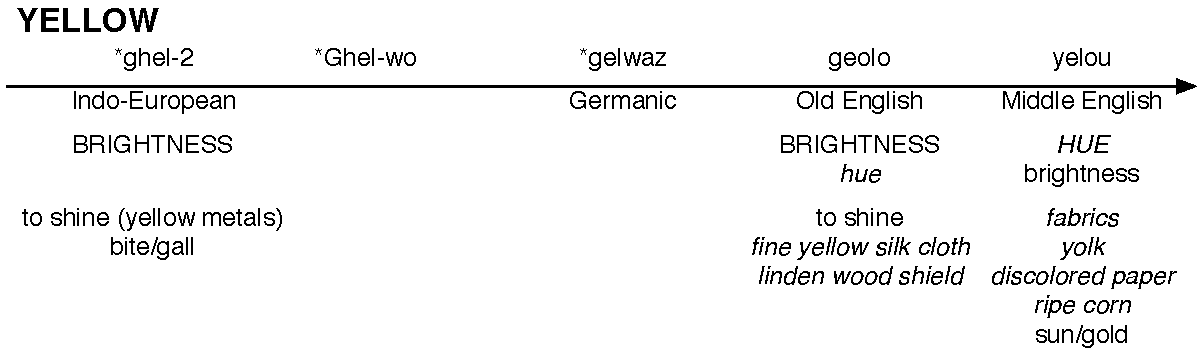
\includegraphics[width=\textwidth]{./selection/figures/history-yellow.pdf}
   \caption[The evolution of the term \textit{yellow} in English]{The
     evolution of the term \textit{yellow} in English. Like almost all
     other basic colour terms, its meaning shifted from brightness to
     hue around the transition from Old English to Middle
     English \citep{casson97shift}.}
    \label{f:ls-history-yellow}
  \end{center}
\end{figure}

The goal of this chapter is to understand and model the competition,
selection and evolution of language strategies for this particular
language phenomenon. Constructing the model consists of the following
steps: identifying and operationalising the language strategies that
are involved in this phenomenon and adding an extra layer of
linguistic selection at the level of language strategies.

\section{Language strategies}

Although in literature the strategies are commonly referred to as
being brightness based or hue based, the hue based strategy does
clearly not ignore the brightness dimension. For example, in
contemporary English the colour category for \textit{yellow} clearly refers
only to light colours whereas \textit{brown} refers to darker colours of a
similar hue. This is commonly attested in literature for a wide range
of languages, including English \citep{sturges95location,
  boynton97insights} and Spanish \citep{lillo07locating}.

The two strategies described above have already been introduced in
\chapref{s:basic-strategy} of this book as being substrategies
of the basic colour strategy: the brightness strategy
and the brightness and hue strategy. Both language strategies
have been operationalised and have been proven to be sufficient to
allow a population of agents to self-organise their own language
system (see \chapref{s:basic-operators} for more details).

\section{Strategy selection}

I can now turn to the main question of this chapter: how can I
orchestrate the coordination of which language strategy to use in such
a way that it optimises expected communicative success but also allows
for a shift from one strategy to another so that I am able to study
the observed phenomenon?

Starting from the observation that colour terms introduced after the
meaning shift only had the hue sense (e.g. \textit{orange} in English), it
seems reasonable to hypothesise that agents keep track of the
\emph{overall success} of a strategy that should be used whenever the
language system is expanded. These overall success rates can also be
used to indicate which strategy to use to expand the language system
when the default strategy is insufficient to tackle the current
communicative challenge. The speaker can use it to use its language in
a more creative way with low risk of failure in communication assuming
that the hearer has a similar ranking for its strategies.

On the other hand, the language system should be able to sustain
enough variability to allow for a shift from one strategy to
another. It should be possible that a strategy becomes successful for
a few terms without hampering overall communicative success so that
the system can reach a tipping point. This suggests that agents should
also keep track of \emph{term-specific success} of a strategy, which
should be preferred over the overall dominant one. The strategy which
has the highest term-specific success for a term, is the \textsc{default
  strategy} which will be used when producing or interpreting a
specific term. A schematic representation of the term-specific scores
is shown in \figref{f:ls-strategies-and-scores}.

\begin{figure}[htpb]
  \begin{center}
    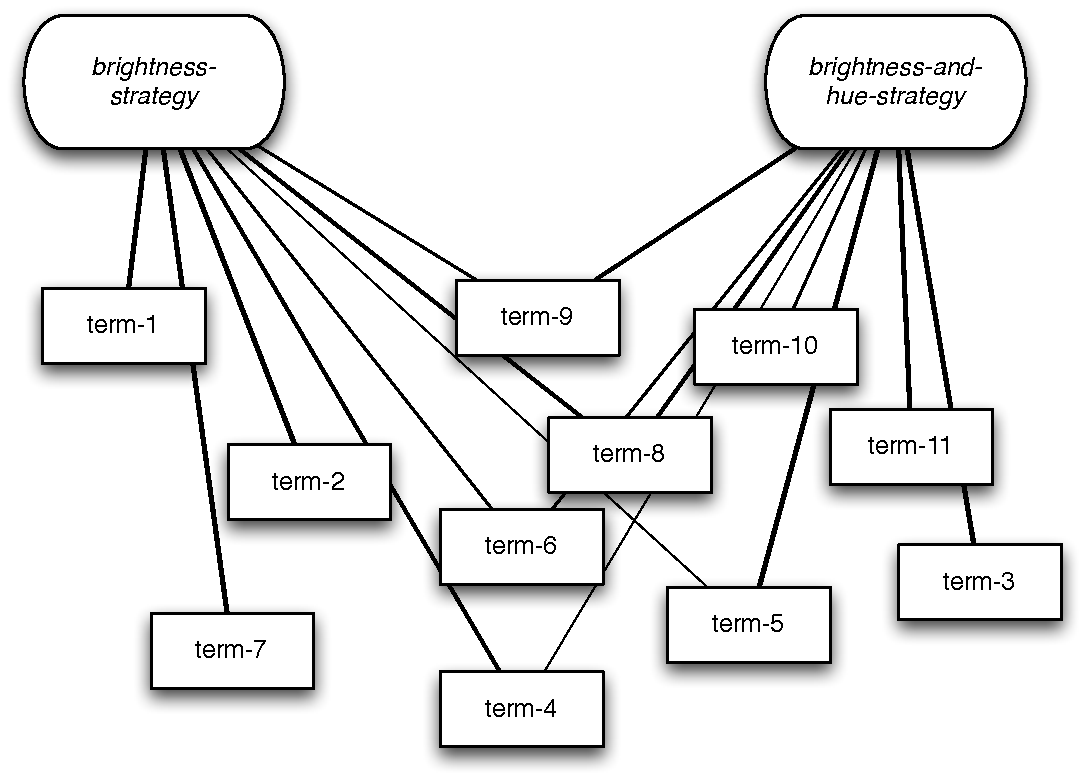
\includegraphics[width=.8\textwidth]{./selection/figures/strategies-scores.pdf}
    \caption[Strategies and their item-specific success
    scores]{Strategies and their item-specific success scores. Each
      term can be used by both language strategies. Depending on the
      communicative context and the term this can lead to
      communicative success which is stored in the item-specific
      success scores. The thickness of the lines represent these
      scores: the thicker the line, the higher the score.}
    \label{f:ls-strategies-and-scores}
  \end{center}
\end{figure}

The term-specific success ensures the language system can sustain
enough variation to allow the shift from one strategy to another. The
overall success increases the expected level of systematicity in the
language system when it needs to be extended as the agent will do so
by using the most conventional and successful language strategy.

\subsection{Implementation of language strategies}

The agents keep track of the \textsc{overall strategy success} of each
language strategy, which reflects its success in previous language
games, regardless of the particular term it was used with.  It is the
average communicative success of the last 50 interactions in which the
strategy was used.

At the same time, the agents keep track of the \textsc{term-specific
  strategy success} of language strategies. This success will be
considered to be the default strategy to produce or interpret this
term. More formally, it is the average communicative success of the
last 50 interactions in which a strategy is used with this specific
term.

\subsubsection{Production and interpretation}

The general procedure to produce an utterance is implemented as
follows. First the speaker tries to use each colour term using the
strategy with the highest term-specific success. When none of these
default interpretations is successful in the current communicative
context, the terms will be reinterpreted using the strategy with the
highest overall success. If this fails as well, the speaker will
reinterpret the terms using the other strategies ordered by
decreasing overall success.

The hearer deploys a similar approach to interpretation, but in most
situations knows which term it needs to interpret. It will do so first
using the strategy with the highest term-specific success. If this
fails, it will reinterpret the term with the strategy with the
highest overall success. If this fails as well, it resorts to the
other strategies ordered by decreasing overall success.

\subsubsection{Alignment}

The agents store the strategy they deployed to produce or interpret a
particular term to update both the overall and the term-specific
strategy success. They also use this strategy to determine which
alignment operators to apply: when the brightness strategy was
deployed only the $L^*$ value of the used category is updated. When
the brightness and hue strategy was deployed, the values of each
dimension are updated (see Section
\ref{s:bcs-adoption-alignment-operators}).

\subsubsection{Invention and adoption}

Whenever an agent feels the communicative pressure to invent a new
colour category, it will use the strategy with the highest overall
success. If this strategy does not work, it will try the other
strategies sorted by decreasing overall success. The hearer will
follow a similar procedure when adopting an unknown form: first it
will try the strategy with the highest overall success and when this
fails, it will try the other strategies ordered by decreasing overall
success.

\section{Experiment on linguistic selection}

In order to focus entirely on the dynamics of the language strategies,
I run an experiment in which the set of basic colour categories is
fixed. This set is equal to the basic focal colours reported for the
Spanish language \citep{lillo07locating}. Which language strategies
the agents should use, is left open. They can choose between either
the brightness or the brightness and hue strategy using
the procedures outlined above. Some terms can be interpreted using
both strategies. The term \textit{amarillo} (`yellow') for example, can be
used both to indicate a light colour or a light colour with a yellow
hue. The contexts consist of three randomly chosen Munsell chips
that have a minimal interstimulus distance of 50 distance units in the CIE
$L^*a^*b^*$ colour space and that should be faithfully reproducible in the
Adobe 1998 RGB colour model.

\subsection{Measures}

\subsubsection{Strategy success}
\is{measures!strategy success}
\is{strategy success|see{measures}}

The strategy success is measured at the population level and is
defined as the average overall strategy success of a particular
strategy in a population of agents.

\subsubsection{Strategy usage}
\is{measures!strategy usage}
\is{strategy usage|see{measures}}

The strategy usage is averaged over all agents in the population. The
strategy usage for an agent is the ratio of the interactions in which
this strategy has been used in the last 50 interactions the
agent was involved in.

\subsubsection{Strategy coherence}
\is{measures!strategy coherence}
\is{strategy coherence|see{measures}}

The strategy coherence ($SC(P)$) is measured at the population level
and is equal to the average scaled strategy coherence of each unique
term ($SC_s(f)$) in the population.

\begin{align}
SC(P) = \frac{\sum_{f \in F} SC_s(f)}{|F|}
\label{e:ls-strategy-coherence-population}
\end{align}

The actual strategy coherence ($SC(f)$) is scaled using the worst-case
coherence ($SC_{wc}$). This ensures the resulting strategy coherence
will result in a value between 1 (full coherence) and 0 (no
coherence).

\begin{align}
SC_s(f) &= \frac{SC(f) - SC_{wc}}{1 - SC_{wc}}
\end{align}

The actual strategy coherence ($SC(f)$) of a term reflects the chances
that two agents will prefer the same strategy for that term in an
interaction. It is based on the distribution of agents over the
different strategies ([$s_i ... s_n$]). The same function is used to
determine the worst-case coherence ($SC_{wc}$), but then using the
worst-case distribution in which the number of agents preferring a
certain strategy is evenly distributed over all available
strategies. For example, in a population of 10 agents and 2 available
strategies, 5 agents will prefer one strategy and the 5 other agents
will prefer the other.

\begin{align}
SC(f) = \sum_{s = s_i}^{s_n}{\frac{s}{|P|}}{\frac{s-1}{|P|-1}}
\end{align}

\subsection{Results}

The resulting dynamics are shown in \figref{f:ls-dynamics} and are
rich and complex. In all runs, the communicative success is as high as
the baseline communicative success (see Figure
\ref{f:bcs-baseline} for comparison) and the agents reach a
high coherence on the default strategies to use for each term in their
repertoire, as indicated by the strategy coherence measure.

Broadly speaking, two situations arise. In one situation, a single
strategy becomes clearly dominant in the population. This could either
be the brightness or the brightness and hue colour strategy, depending
on small fluctuations in the early choices of the population (Figure
\ref{f:ls-one-winner}). But I have also observed situations where one
strategy becomes dominant first (for example, the brightness
  strategy) to be overtaken later by the other strategy (in this case
the brightness and hue strategy, as seen in the history of
English (\figref{f:ls-competition}). In this case, the two
strategies continue to coexist in this case. Brightness is still used
in circumstances when there is a word for which the default strategy
is still the brightness strategy.

\begin{figure}[htbp]
\begin{center}
\subfigure[]{
  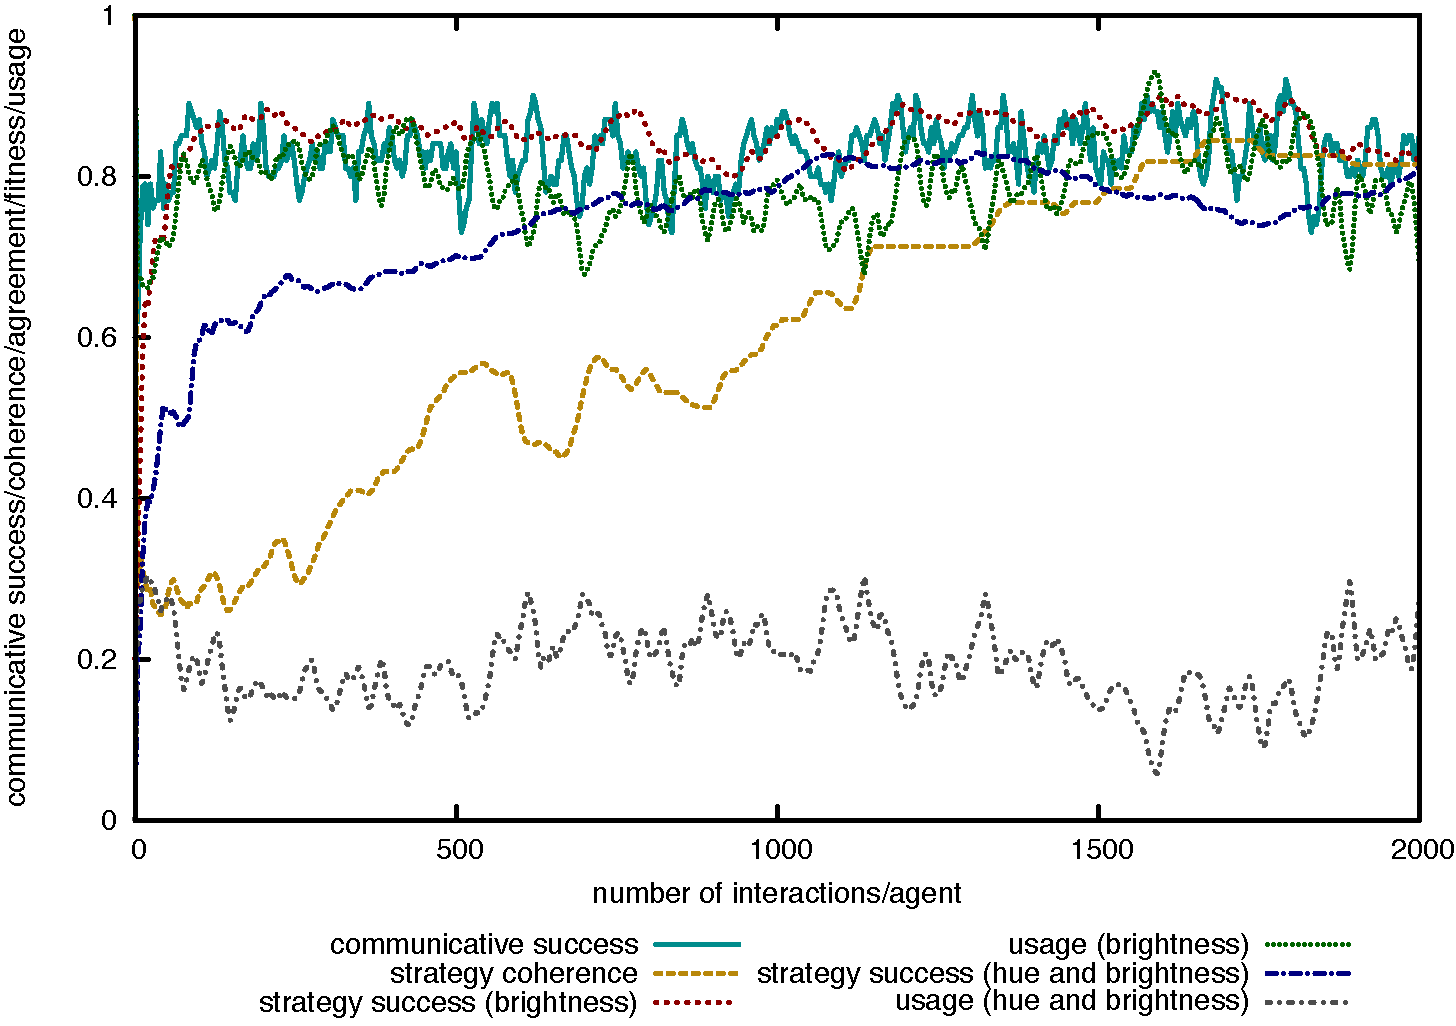
\includegraphics[width=.8\textwidth]{./selection/figures/strategies-one-winner.pdf}
  \label{f:ls-one-winner}
} 
\subfigure[]{
  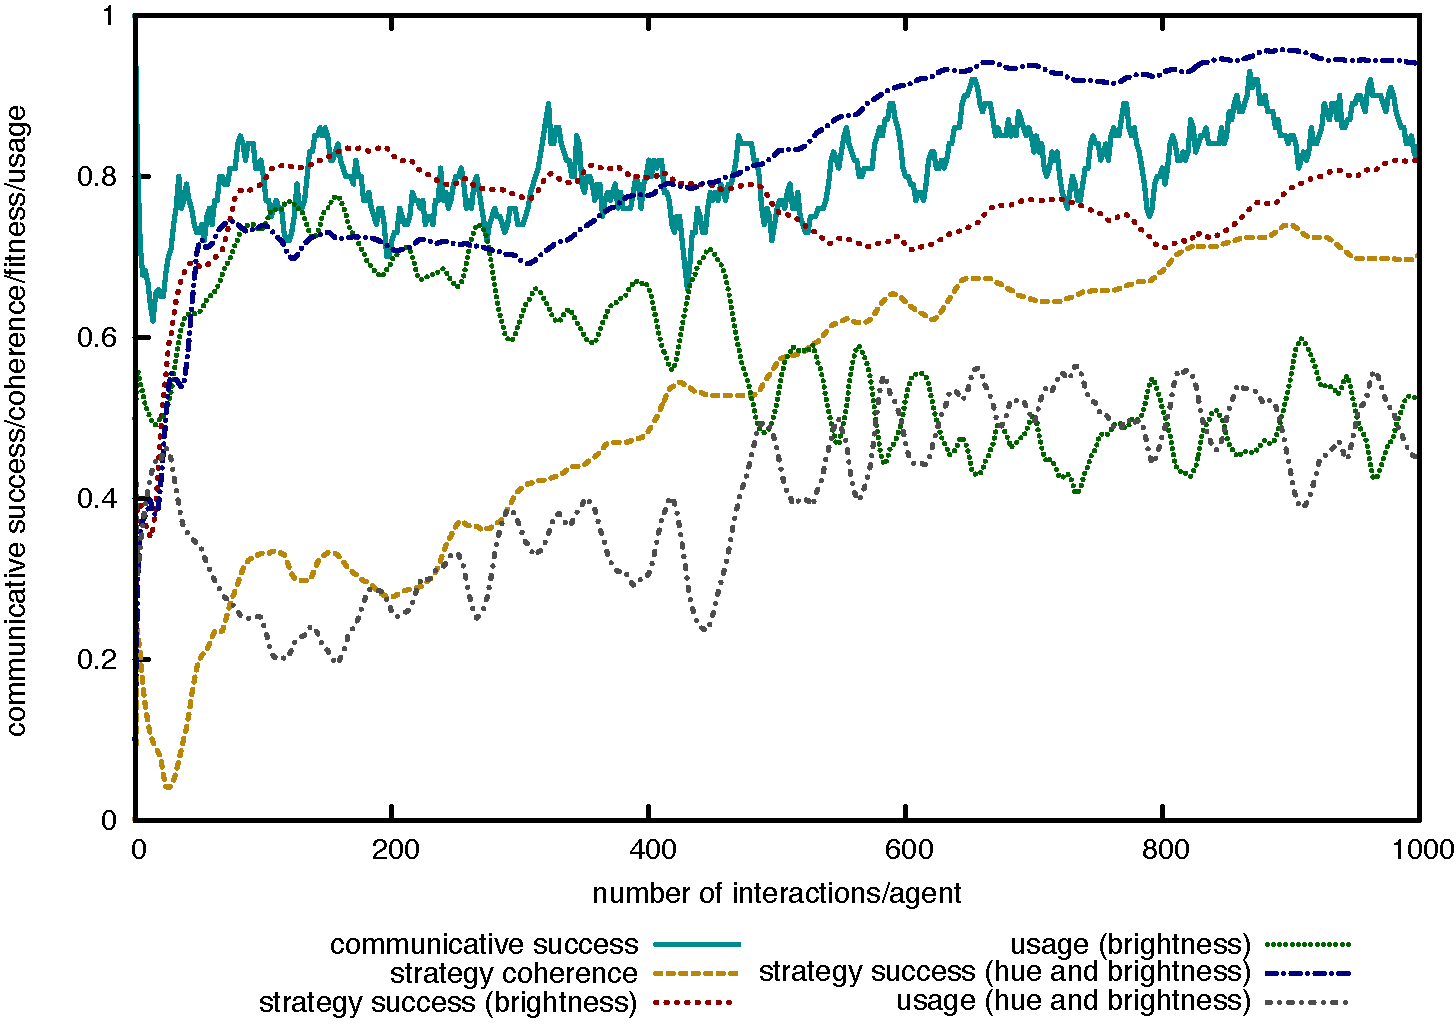
\includegraphics[width=.8\textwidth]{./selection/figures/strategies-competition.pdf}
  \label{f:ls-competition}
}
\end{center}
\caption[Resulting dynamics of the linguistic selection of
strategies]{The resulting dynamics of the linguistic selection of
  strategies. In \subref{f:ls-one-winner} the brightness
    strategy becomes entirely dominant and is used significantly
  more, whereas in \subref{f:ls-competition} one strategy overtakes
  the dominant one which is reflected in the respective use of each
  strategy.}
\label{f:ls-dynamics}
\end{figure}

\section{Selective advantage}
\label{s:ls-selective-advantage}
\is{language strategy!selective advantage of}

The expected communicative success for a particular language strategy
is highly dependent on the linguistic challenges in which it is
deployed. By manipulating these challenges, one can try to determine
the expected communicative success and to find in which type of
contexts one strategy has a selective advantage over the others.

To study the impact of the linguistic challenges on the expected
communicative success, I have designed two types of artificially
constrained linguistic contexts. In the first type, the \textsc{constant
  brightness contexts}, all samples in the contexts share the same
lightness value, so they only differ in hue. In the second type, the
\textsc{constant hue contexts}, the samples are all different shades of
grey, so they only differ in lightness. By exploring different
mixtures of these two types of contexts, I can establish environmental
constraints in which one strategy would become more successful than
the other.

\subsection{Experiment}
\label{s:ls-selective-advantage-experiment}

In this experiment I will compare three \textsc{basic language
  strategies}. In addition to the brightness and the
brightness and hue strategy, I will also study the hue
  strategy in which only the two hue dimensions ($a^*$ and $b^*$ in
the CIE $L^*a^*b^*$ colour space) are taken into account. The agents
start from a predefined lexicon based on Spanish
\citep{lillo07locating}, the contexts consist of 4 Munsell chips
with a minimal interstimulus distance of 10 distance units in
the CIE $L^*a^*b^*$ colour space. The chips are limited to the ones
that are reproducible in the Adobe 1998 RGB colour model. The ratio
of constant hue to constant brightness contexts is controlled through
the hue difference parameter.

\subsubsection{Results}

The results are shown in \figref{f:ls-selective-advantage} and
indicate the resulting strategy success after 10k interactions. The
communicative success of brightness strategy is optimal when
there are no contexts in which the hue is constant, but the success
drops when more contexts of constant brightness are present in the
challenges. The opposite is true for the hue strategy which has
its optimal success when the contexts are variable in hue. This
success decreases as the ratio of contexts which are of constant hue
increases. The brightness and hue strategy becomes more
successful than the brightness strategy when 3 out of 10
contexts are of constant brightness. This shows the selective
advantage of one strategy over the other.

\begin{figure}[htbp]
\begin{center}
  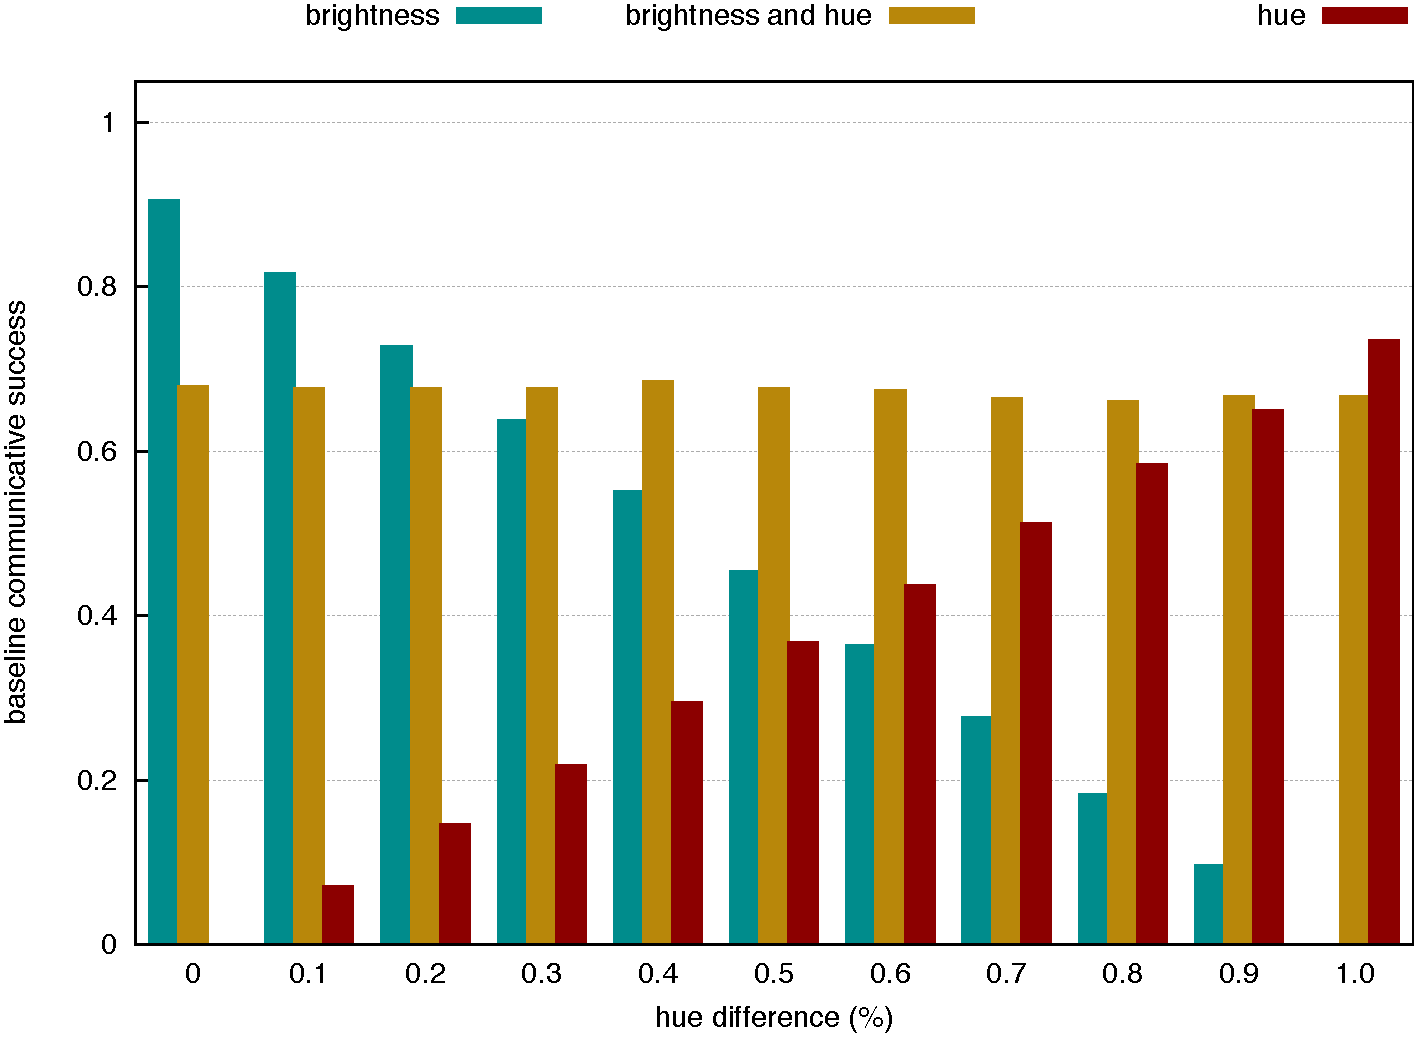
\includegraphics[width=.8\textwidth]{./selection/figures/selective-advantage.pdf}
\end{center}
\caption[Selective advantage of basic colour strategies]{Selective
  advantage of the brightness, hue and brightness and
  hue strategies. The baseline communicative is compared in
  mixtures of two types of contexts. The hue difference reflects the
  ratio of constant hue to constant brightness contexts.}
\label{f:ls-selective-advantage}
\end{figure}

It might seem surprising that brightness strategy is more
successful than the brightness and hue in black-and-white
contexts as the latter uses more information. This is due to the
semantics in production which considers only the category that is the
most similar to the topic. When all dimensions are relevant, only the
three achromatic colour categories (black, grey and white) can be used
as these are the most similar to the black and white samples. When
only one dimension is deemed relevant, each category will cover a
small part of the axis between white and black, resulting in higher
communicative success.

\section{Conclusion}
\label{s:ls-conclusions}

I have explored how agents can align their choice of which language
strategy to use through linguistic interaction. I have hypothesised
that there should be a second level of selection in which agents keep
track of the overall success of the language strategies they are
using. This level of selection can be used to increase the level of
systematicity when the language system needs to be expanded and to
minimise potential misunderstandings when certain terms are used in an
unconventional way. At the same time language systems should be able
to sustain enough variation to allow for shifts in dominance from one
strategy to another. This is why agents should also keep track of
which strategy is most commonly used with a particular item. I have
shown how these principles can lead to a model in which agents reach
high coherence in what strategies to use, but that is also open as to
which strategy becomes dominant. The same model is also capable of
replicating the observed phenomenon presented in the introduction of
this chapter. I have also shown that the selective advantage of one
strategy can be systematically studied by manipulating the
communicative contexts in which it is deployed.